%************************************************
\chapter{Problem Statement}\label{ch:problemstatement}
%************************************************

Event subscription is an essential part of event-driven architectures and must consequently be considered when using events in business processes.
While the use of external events is an active topic in research, most approaches only briefly discuss the subscription mechanism and use the \acs{BPMN}~semantics for orientation.
\todo[inline]{ref}
Though event subscription is not directly addressed in the BPMN~specification, the descriptions on intermediate events state:

\medskip
\textit{"For Intermediate Events, the handling consists of waiting for the Event to occur. Waiting starts when the
Intermediate Event is reached. Once the Event occurs, it is consumed."}~\cite{bpmnspec},~p.~440

\medskip \noindent The usual interpretation of this excerpt is that the subscription to the event takes place as soon as the event gets enabled, the un-subscription when the event terminates.
\todo[inline]{I need to work with a precise lifecycle}
As pointed out by Mandal~et.~al.~\cite{mandal:2017}, these subscription semantics significantly limit the flexibility of using events in business processes and can cause undesired behavior and fault.
Due to the strict temporal order between event subscription, occurrence and un-subscription as required by the publish-subscribe paradigm, any events that occur before the enabling of the event element will be ignored by the process execution.
That reduces the timespan for events to occur to a potentially small part of the total execution time and means that crucial events might be missed which can delay or block a process execution unnecessarily.

In the following section, the problem is further illustrated at the example of two sample scenarios.
The observed situations then lead to the definition of \textit{Event Occurrence Scenarios} and the derivation of a set of requirements that must be fulfilled by a mechanism for flexible event subscription in business processes.

\section{Motivating Examples}\label{ch:motivatingexamples}
% some has been mentioned in the introduction
%illustrate the complexity

To allow a better understanding of the issue, event-driven use-cases from two different domains are presented in the following.
The cases are revealed through their standard BPMN representation.
It is illustrated, why the time of event subscription is of great importance which motivates to study the mechanics and implications of event subscription in business processes.

\paragraph{Delay of a logistics process}
The first example~(\autoref{fig:example-eurotunnel}) is taken from the logistics domain and shows a truck transport that has to cross the English Channel.
The truck driver receives the transport plan for his next tour from France to the UK. By default, the company crosses the Channel using the Eurotunnel, an underground train connection between London and Paris.

\begin{figure}[]
	\myfloatalign
	{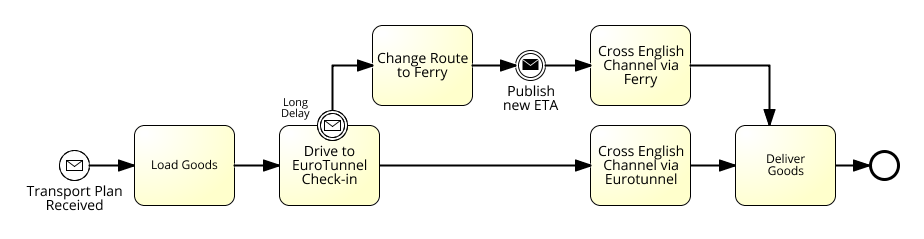
\includegraphics[width=1\linewidth]{chapters/requirements/Eurotunnel-simplified.png}}
	\caption{BPMN Model of a Logistics Process using events for route~optimization~(Example 1.1)}
	\label{fig:example-eurotunnel}
\end{figure}

After loading the goods at the factory, the truck will head towards the check-in location of the Eurotunnel.
If everything runs on schedule, the truck crosses the channel on the train and then delivers the goods in Great Britain.
Alternatively, the process considers a route using the ferry from Calais~(FR) to Dover~(UK).
The Eurotunnel administration publishes delay information approximately every 30~minutes through an RSS feed on their website. While it mostly operates on schedule, delays ranging from 15~minutes to several hours occur regularly. It can happen that new information is not published for multiple hours.
Significant delay events (delay~>~30~minutes) are received through a boundary catching message event attached to the activity \textit{Drive to Eurotunnel Check-In}. The boundary event is interrupting, hence the activity is canceled if a delay occurs.
The transport continues towards the ferry terminal and crosses the English Channel over sea. After crossing the channel, the goods are delivered to the recipient.
\todo[inline]{show a cep query for that scenario to make it more precise}

As interpreted from the BPMN specification, the subscription to the boundary event is issued as soon as the related activity is enabled.
Given that events arrive every 30~minutes, there can be a gap of up to half an hour, before the first information becomes available.
In the worst cases, when data isn't published for several hours, this gap will be even bigger.
Let's consider a very busy weekday; A technical fault occurred in the tunnel earlier that day and the train runs 3 hours behind schedule.
The last information on the RSS feed was published at 2:35\,pm. At that time the truck driver is still in the process of loading goods, finishing the activity at 2:40\,pm.
Following the process definition, the driver now departs towards the Eurotunnel check-in.
The system publishes updated information at 3:15~pm, operations are still 2:30\,h behind schedule. The message gets received through the process and the truck driver takes the alternative route to the ferry, but only after heading to the Eurotunnel for 35~minutes. The late change of plans causes an unnecessary delay to the shipment.

\begin{figure}[]
	\myfloatalign
	{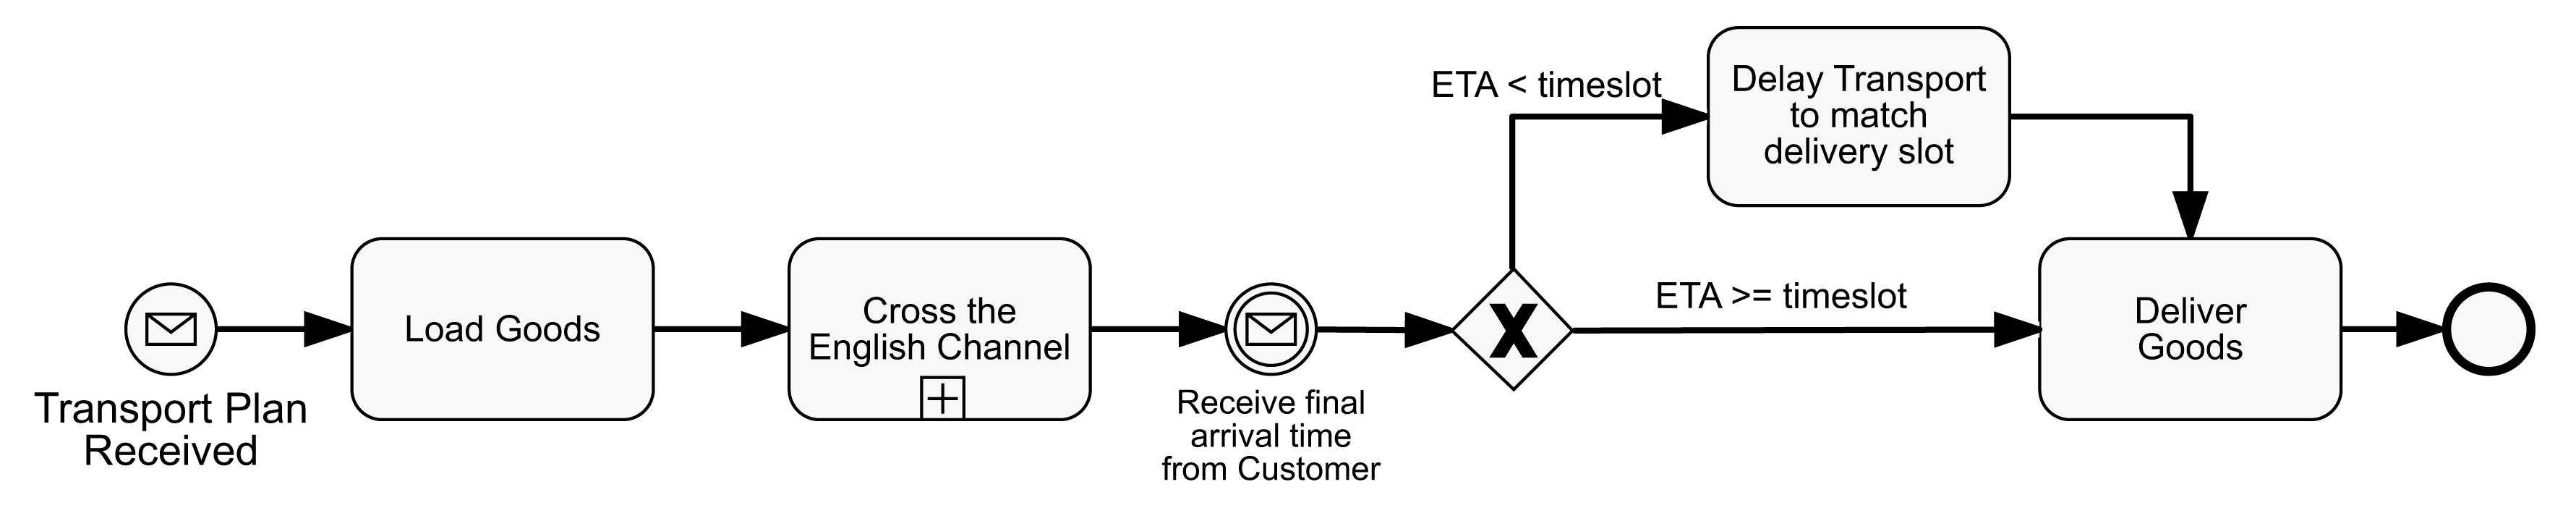
\includegraphics[width=1\linewidth]{chapters/requirements/Eurotunnel_part2.png}}
	\caption{Transport via English Channel that is timed to a delivery~slot~(Example~1.2)}
	\label{fig:example-eurotunnel-part2}
\end{figure}

\autoref{fig:example-eurotunnel-part2} is an extension of the the transport process.
In logistics, it is common that a delivery cannot be accepted at an arbitrary time. Instead, the receiving party assigns delivery windows to the transport company.
The transport must arrive during the given time window, otherwise the delivery cannot be completed.
After crossing the English Channel, the process model shows the catching of a message event containing the desired final arrival time at the factory. There is an agreement with the factory, that the delivery slots will be approved 2~hours before the expected arrival.
If the current ETA of the transport is greater or equal to the arrival time, the driver will head to the drop-off point immediately. If the transport is ahead of schedule, the driver will have to delay the delivery to match the time window.

The presented process model illustrates another complexity of using events in processes. Again, the listening to the announcement of a delivery window will start when the event element is enabled, in this case after crossing the English Channel. 
Until an event has been received, the process will not continue. 
Much worse: if the receiving party sends out the arrival time information too early, \ie~while the truck is crossing the channel, the event is missed. If it is not issued again, the process cannot receive a message and will get stuck indefinitely waiting to catch the event.

Neither of the two presented catch events allow for an efficient and reliable execution of the process. They can cause unnecessary delays and even blocking of the process execution.

\todo[inline]{Consider more possible event occurrence times to prepare for the next chapter}

\paragraph{Up-to-date shipping information for an order}
\begin{figure}[]
	\myfloatalign
	{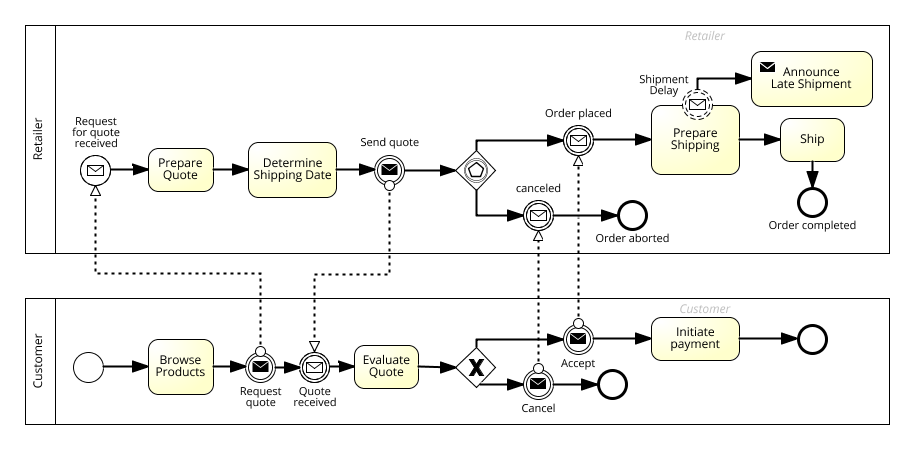
\includegraphics[width=1\linewidth]{chapters/requirements/Retail-Order.png}}
	\caption{Model of a retail order management process (Example 2)}
	\label{fig:example-order}
\end{figure}

A~similar situation can be observed in the order-management process depicted in \autoref{fig:example-order}.
It describes the interaction between customer and seller in a traditional distance retail scenario: After browsing the product catalog, the customer requests a quote for the articles he or she is willing to buy.
The retailer makes an offer including an approximation of the expected shipment date and sends it to the customer. That quote is then either accepted or not and the payment is issued if necessary.
Once the retailer is informed about the placement of the order, the products are packed and shipped as soon as possible.
For articles that are not currently in stock, the retailer must await the shipment from the factory. If any of the factory-shipments is delayed, the retailer cannot ship in time and will announce a delayed shipment date to the customer.
This situation is modeled through a non-interrupting boundary event attached to the \textit{Prepare Shipping} activity, which triggers the sending of the updated shipment date to the customer.

The process shows a number of similarities, but also differences in terms of event-use when compared to the logistics process in Example~1.
At first we look at the three intermediate catch events, \textit{Quote~received}, \textit{Order~canceled} and \textit{Order~placed}.
In each of the cases, the event to be caught is the direct response to a message that was sent right before. While the process will also enter a waiting state until the response arrives, that waiting is not to be interpreted as an unnecessary delay to the process execution.
Other than in Example~1.2\,(\autoref{fig:example-eurotunnel-part2}), there is nothing useful to do before the response is received.
It is furthermore worth noting that the response messages cannot be missed, because the message catch event immediately follows the message send event.

A different situation holds for the boundary event \textit{Shipment Delay}.
While the subscription to a Eurotunnel event can be issued at any time, it does not depend on any process data, the shipment delay has to be observed for each product that is part of the order. A subscription can therefor not be executed before the activity \textit{Prepare~Quote} has terminated. \todo[inline]{show a cep query for that scenario to make it more precise}
Conforming to the definition of the process, the system will listen to shipment delays once the activity \textit{Prepare~Shipping} is enabled and therefor much later than possible.
Any events that occur after the completion of \textit{Prepare~Quote} but before \textit{Prepare~Shipping}, cannot be considered in the process execution and the customer will not be informed about a possible late shipment. That will, for instance, concern events that occur while the customer makes the decision about accepting or canceling the order.

% The first of these three follows the \textit{Send/Receive} Service Interaction Pattern. \todo[inline]{missingref}
% Two parties interact 

\medskip \noindent 
The two presented examples have illustrated the complexity of using events in business processes, especially when all possible event occurrence times are taken into consideration.
Differences have been pointed out as to how exactly the event is placed in the process, if it waits for a direct response to an earlier request or if the event occurrence is unrelated to the execution of that very process.
Motivated by this complexity and the possible implications, it is the goal of this work to evaluate the capabilities of BPMN and to present a concept for the flexible handling of event subscription in business processes.


\section{Event Occurrence Scenarios and Time of Subscription}\label{ch:ps:eos}
Given the motivating examples, a generic set of \textit{Event Occurrence Scenarios} is defined in this section. 
Each of the scenarios represents a real-world situation and process implementations need to be capable of handling them to avoid negative effects.

\medskip \noindent
The dominant variable to consider is the event occurrence time.
According to the BPMN specification, it is possible to catch an event if it occurs after the event element is enabled. As shown before, it is often impossible to control occurrence time and events do occur outside of the listening time intervals.
An \ac{EOS} describes the time of event occurrence in relation to a specific step in process or engine execution.
The life-cycle of a process within a process engine is explained in \autoref{ch:bg:bpm} and taken as reference. It is assumed that the process and event engine are configured and running.
An event is considered to always occur before or after a life-cycle step or in between two consecutive steps. 
Given the life cycle steps \textit{process deployment}, \textit{process instantiation} and \textit{event enabling}, the following occurrence scenarios are distinguished in this work:
% they have an implicit temporal order

\begin{aenumerate}
	\item[$EOS_{1}$] While the BPMN event element is enabled
	\item[$EOS_{2}$] The event does not occur
	\item[$EOS_{3}$] Between process instantiation and \\the enabling of the BPMN event
	\item[$EOS_{4}$] Between process deployment and \\process instantiation
	\item[$EOS_{5}$] Before process deployment
\end{aenumerate}\label{def:occurrence-times}
% they are ordered this way to be in line with the assessment chapter

\begin{figure}[]
	\myfloatalign
	{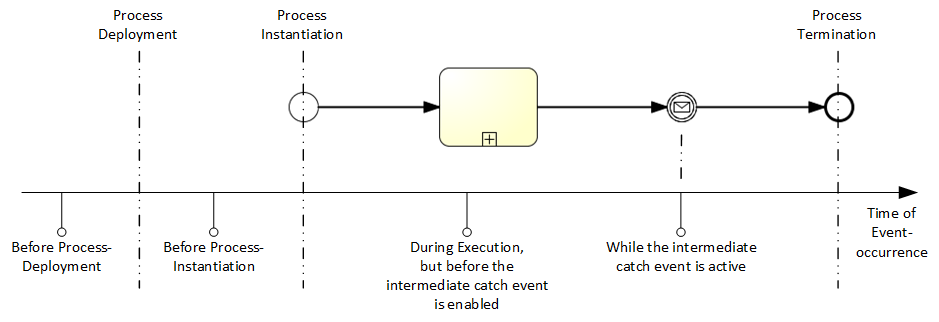
\includegraphics[width=1\linewidth]{chapters/requirements/timeline-event-occurrence.png}}
	\caption{Possible event occurrence times in relation to a process execution life cycle}
	\label{fig:occurrence-timeline}
\end{figure}\todo[inline]{improve figure: include EOS notions, save space, ?}

An overview of the EOSs and the related life-cycle steps is provided in \autoref{fig:occurrence-timeline}, which uses a time-line to illustrate the possible event occurrence times.
The model deliberately excludes event occurrences after termination of the event element, because that would presume that there is no more interest in the event as the execution flow continued on another branch. Otherwise, the process will remain in waiting state until the event occurs.

\todo[inline]{add a back reference to the examples. In example XY, events can occur before... whereas in example...}

As introduced in \autoref{ch:bg:cep}, there is a strict temporal order between event subscription, reception and un-subscription.
To catch an event that occurs as described in any of the EOSs, the related subscription operation has to be executed before the start of the time interval associated with the EOS.
On that basis, the latest possible event subscription time can be derived from each event occurrence scenario and is as follows:
\textit{before process deployment}~($EOS_{5}$), \textit{during process deployment}~($EOS_{4}$), \textit{at process instantiation}~($EOS_{3}$) and when the \textit{BPMN event element is enabled}~($EOS_{1}$).

It is important to highlight that the subscription to an event source can depend on additional context information or process data, which can be a significant limitation to the possible subscription time.
That situation is illustrated in \textit{Example~2}~(\autoref{fig:example-order}), where the subscription to the shipment delay information cannot be executed before the \textit{Prepare~Quote} activity is completed.
More generally put, a \textit{subscription~dependency} is defined as follows:

\begin{description}
	\item[Subscription Dependency]
	The subscription operation is \textit{dependent}, if any of its parameters, for instance the event query, contains a variable value that has to be determined at the time of subscription.
	The value might reference a piece of information from the process instance context, an engine-wide piece of data or external information.
	In case of a dependence, the subscription cannot be issued before the associated information is available.
\end{description}

If a subscription dependency resolves before the process execution reaches the event element, it should still be possible to flexibly chose the subscription time in the process.
For that reason, in addition to the four subscription-time options presented earlier, an additional option \textit{at any time during process execution} must be available.


\section{Requirements Definition}\label{ch:requirements}
The previous sections have exemplified how the BPMN execution semantics and notation capabilities limit users when using events in business processes. 
Now, these shortcomings are formalized into an initial set of requirements additional to the features offered by BPMN.
They build the foundation for enhancing BPM solutions towards flexible event subscription management~(\autoref{ch:flexibleeventsubscription}).
Before that, the formal requirements will be used to evaluate the capabilities of current Process Management Solutions~(\autoref{ch:assessment}), which results in an additional set of requirements \textit{R4-R6} presented in \autoref{ch:ass:reqextension}.

%\medskip \noindent
%It shall be noted that the requirements \textit{R2.2} and \textit{R3} introduced in this chapter have also been pointed out by Mandal~et.\,al. in their work on early subscription and event buffering\,\cite{mandal:2017}.
%Note that the need for flexible event subscription has also been pointed out by Mandal~et.\,al. in their work on early subscription and event buffering\,\cite{mandal:2017}. The authors follow a similar line of argumentation and also specify the requirement for a flexible time of subscription and event buffering.


%Andreas: Dein Kommentar im Text sollte eigentlich überflüssig sein, weil du die Begrifflichkeit zuvor in Kapitel 2 geklärt haben solltest. Hier würde ich maximal einen kurzen Recap mit Verweis auf Ch.2 machen.
\todo[inline]{by event I usually mean event from a cep pub/sub event source. The requirements relate to external intermediate message events. A limitation that is made in accordance with the motivated scenario. though some of the aspects might apply to other types of eventy, like the start event.}


\paragraph{R1: Subscription Fundamentals}

\begin{description}
	\item[R1.1 Subscription to an Event Source:]
	To enable the reception of events from a publish/subscribe event source, the subscription operation must be part of the execution flow. 
	In accordance with the obligatory temporal order of operations, the subscribe operation must happen before an event can be received and/or the un-subscription takes place.
	\item[R1.2 Un-subscription:]
	As soon as events from the source must not be received anymore, an un-subscription has to take place.
	\item[R1.3 Availability of Information:]
	For each event that is used in a business process, all information necessary to execute an event subscription in the given execution environment must be available.
	That information generally includes the event query, the address of an event processing platform and auxiliary information to establish the communication, for instance authentication data.
	%While the event query is associated to a specific event element and must therefor be part of the process model, the process platform information might be valid for potentially all processes and can be made available through a global data store.
	\item[R1.4 Variables in Event Queries] 
	To adapt an event subscription to execution- or time-specific information, variables can be utilized as part of the query string.
	At the time of event subscription, these variables must be replaced their current values before the subscription is executed.
	
\end{description}

\paragraph{R2: Event Subscription Time}

\begin{description}
	\item[R2.1 Explicitness:] 
	For each event that is used in a business process, it must be possible to derive the time of event subscription from the process model. The time of subscription may either be explicitly stated or defined implicitly.
	\item[R2.2 Flexibility:] 
	The time of subscription can be influenced independently from the place the event element takes in the model. Timing options are made available to catch events according to any of the event occurrence scenarios EOS1, EOS3, EOS4 and EOS5. 
	Consequently, the options must include but are not limited to the subscription before process deployment, during  pr. deployment, at process instantiation, subscription at an arbitrary but explicit time during process execution or when the event element is enabled.
	Thereby, also events that occur after the time of subscription, but before the event element is enabled shall be available to be consumed.~(cf.\,\cite{mandal:2017})
	%By that means, the variability of the time of event occurrence can be specifically addressed in the process model and unnecessary delay or blocking of the execution can be reduced.
	\item[R2.3 Awareness of Subscription Dependencies:]
	The additional flexibility provided through \textit{R2.2} is limited by the use of variables in event queries~(\textit{R1.3}) and the implicit dependencies on context information.
	The execution environment must only allow a subscription time after the resolving of all dependencies.
	
	Dependencies can exist within a certain process instance, for example when an information from a local DataObject is referenced in a query. In more complex scenarios, the subscription might depend on data from other process instances or even other processes which must first be obtained.
\end{description}


\paragraph{R3: Event Buffering}

\begin{description}
	\item[R3.1 Buffering Principle:]
	%To make all events since the subscription time available during process execution, matching events need to be stored temporarily.
	As introduced by \textit{R2.2}, an indefinite time can pass between the time of subscription and the consumption of the event.
	While the subscription operation generally assures that the event is received, it is necessary to temporarily store it until the consuming element is reached.
	
	This temporary storage is referred to as an \textit{Event~Buffer}.
	The storage must be designed to fulfill the semantics demanded by \textit{R2.2} which means that any event that occurs after the time of event subscription must be available to consume.
	
	\item[R3.2 Buffer Scope:]
	The flexible event subscription time~(\textit{R2.2}) allows an event subscription after process instantiation, but also before process instantiation or deployment.
	It can be inferred that an event buffer operates either in the scope of a process instance, a process definition, or in the scope of the complete execution environment.
	To implement all event subscription times stated in \textit{R2.2}, the execution environment must support event buffering in each of the three scopes. 
	The provided concept must make clear to the user, which scope is referenced at any point in time.
	
	\item[R3.3 Buffer Policies:]
	The behavior of a buffer in any occurring situation must be specific.
	The parameters necessary to specify the behavior are referred to as \textit{Buffer Policies}, following the notion chosen by  Mandal~et.\,al.\,\cite{mandal:2017}.
	
	\item[R3.3.1 Lifespan Policy:]
	Given that the time between the event subscription and its consumption may be indefinitely long, process designs can require to limit the maximum time an event is held in the buffer.
	%A parameter must be offered to specify this timespan.
	
	\item[R3.3.2 Consumption Policy:]
	Requirement \textit{R3.2} implies that buffers can be shared among process instances of the same process and other processes.
	In this scenario, it needs to be defined if an information is consumed from the buffer upon retrieval, or if the information remains in the buffer for other participants to access. 
		
	\item[R3.3.3 Size Policy:]
	Provided that multiple events can occur between the time of subscription and the enabling of the event element, it must be specified for each buffer, how many events should be stored for later consumption.
	%In basic scenarios, where a buffer is only accessed a single time by one catch event in one process instance, a fixed buffer size of one element will be sufficient. However, if a buffer is accessed multiple times or shared among instances, the buffer size may vary between~1~and infinity.
	
	\item[R3.3.4 Retrieval Order Policy:]
	If multiple events are stored in the buffer~(\textit{R3.3.3}), it must be defined, in which order the events are provided for consumption. 
	%The order can be chosen as \textit{First in first out}~(FIFO) or \textit{Last in first out}~(LIFO) 
	
\end{description}



